\subsection{\texorpdfstring{Inverse Image of a \(\tau\)-Extension}{Inverse Image of a \textbackslash tau-Extension}}

Let G and \(G'\) be groups. Let F be an abelian group, and let \(\tau: G \to \text{Aut}(F)\) and \(u: G' \to G\) be group homomorphisms. Consider the group homomorphism \(\tau' = \tau \circ u: G' \to \text{Aut}(F)\) , and denote by \(\Gamma'\) the fiber product \(\Gamma \times_{G} G'\) with respect to \(\pi\) and u (I, §4, No.~8, p.~46). It is the subgroup of \(\Gamma \times G'\) consisting of the pairs \((\gamma, g')\) such that \(\pi(\gamma) = u(g')\) . Let \(\iota': F \to \Gamma'\) be the group homomorphism given by \(\iota'(\alpha) = (\iota(\alpha), e)\) for \(\alpha \in F\) , and denote the second projection by \(\pi': \Gamma' \to G'\) . Then the morphism \(\iota'\) is injective, the morphism \(\pi'\) is surjective because \(\pi\) is, and the image of \(\iota'\) coincides with the kernel of \(\pi'\) . Moreover, for every \(\alpha \in F\) and \(\gamma' = (\gamma, g) \in \Gamma'\) , we have the relations

\[
\gamma^ {\prime} \iota^ {\prime} (\alpha) \gamma^ {- 1} = (\gamma , g) (\iota (\alpha), e) (\gamma , g) ^ {- 1} = (\iota (\tau (\pi (\gamma)). \alpha), e) = \iota^ {\prime} (\tau^ {\prime} (\pi^ {\prime} (\gamma^ {\prime})). \alpha)
\]

Consequently, \((\Gamma', \iota', \pi')\) is a \(\tau'\) -extension of \(G'\) by F; we call it the inverse image of E by u and denote it by \(u^{*}(\mathcal{E})\) . The first projection is a group homomorphism \(\varphi : \Gamma' \to \Gamma\) that we call canonical.

PROPOSITION 1. --- The following diagram commutes:

\[
\begin{array}{c} \mathrm{F} \xrightarrow {\iota^ {\prime}} \Gamma^ {\prime} \xrightarrow {\pi^ {\prime}} \mathrm{G} ^ {\prime} \\ \Big \| \qquad \qquad \qquad \Big \downarrow \varphi \qquad \qquad \Big \downarrow u \\ \mathrm{F} \xrightarrow {\iota} \Gamma \xrightarrow {\pi} \mathrm{G}. \end{array}\tag{2}
\]

Moreover, if \(\mathcal{E}_1' = (\Gamma_1', \iota_1', \pi_1')\) is a \(\tau'\) -extension and \(\varphi_1: \Gamma_1' \to \Gamma\) is a group homomorphism such that the diagram

\[
\begin{array}{c} \mathrm{F} \xrightarrow {\iota_ {1} ^ {\prime}} \Gamma_ {1} ^ {\prime} \xrightarrow {\pi_ {1} ^ {\prime}} \mathrm{G} ^ {\prime} \\ \Big \| \qquad \qquad \qquad \Big \downarrow \varphi_ {1} \qquad \qquad \Big \downarrow u \\ \mathrm{F} \xrightarrow {\iota} \Gamma \xrightarrow {\pi} \mathrm{G} \end{array}
\]

commutes, then there exists a unique morphism \(\psi\) of \(\tau'\) -extensions from \(\mathcal{E}_1'\) to \(u^*(\mathcal{E})\) such that we have \(\varphi_1 = \varphi \circ \psi\) .

The commutativity of the first diagram follows from the definition of \(\varphi\) . The existence and uniqueness of \(\psi\) follow from Lemma 2 below.

Lemma 2. --- Let \(F_{1}^{\prime}\) be an abelian group, and let \(w : F_{1}^{\prime} \to F\) and \(\tau_{1}: G^{\prime} \to \operatorname{Aut}(F_{1}^{\prime})\) be group homomorphisms such that

\[
w (\tau_ {1} (g) (f)) = \tau (u (g)) (w (f))
\]

for every \(f \in \mathrm{F}_1'\) and \(g \in \mathrm{G}'\) . Let \(\mathcal{E}_1' = (\Gamma_1', \iota_1', \pi_1')\) be a \(\tau_1\) -extension of \(\mathrm{G}'\) by \(\mathrm{F}_1'\) and \(\varphi_1: \Gamma_1' \to \Gamma\) a group homomorphism such that the following diagram commutes:

\pandocbounded{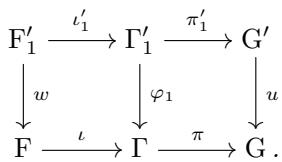
\includegraphics[keepaspectratio]{images/part002_e5b6b945.jpg}}

Then there exists a unique group homomorphism \(\psi : \Gamma_1' \to \Gamma'\) such that the diagram

\pandocbounded{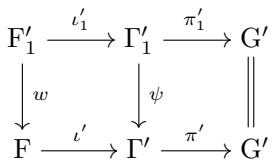
\includegraphics[keepaspectratio]{images/part002_7bcd6e81.jpg}}

commutes and \(\varphi_{1} = \varphi \circ \psi\) .

If the group homomorphism \(\psi : \Gamma_1' \to \Gamma'\) has the desired properties, then it satisfies the relations

\[
\psi (\gamma) = (\varphi \circ \psi (\gamma), \pi^ {\prime} \circ \psi (\gamma)) = (\varphi_ {1} (\gamma), \pi_ {1} ^ {\prime} (\gamma))
\]

for every \(\gamma \in \Gamma_1'\) . Conversely, the group homomorphism from \(\Gamma_1'\) to \(\Gamma \times G'\) defined by \(\gamma \mapsto (\varphi_1(\gamma), \pi_1'(\gamma))\) has values in the fiber product \(\Gamma \times_G G'\) because \(\pi \circ \varphi_1(\gamma) = u \circ \pi_1'(\gamma)\) for every \(\gamma \in \Gamma_1'\) .

COROLLARY 1. --- Let \(E_{1}\) and \(E_{2}\) be \(\tau\) -extensions of G by F, and let \(\psi\) be a morphism of \(\tau\) -extensions from \(E_{1}\) to \(E_{2}\) . Denote by \(\varphi_{1}\) (resp. \(\varphi_{2}\) ) the canonical homomorphism for \(u^{*}(\mathcal{E}_{1})\) (resp. \(u^{*}(\mathcal{E}_{2})\) ). Then there exists a unique morphism of \(\tau'\) -extensions from \(u^{*}(\mathcal{E}_{1})\) to \(u^{*}(\mathcal{E}_{2})\) , denoted by \(u^{*}(\psi)\) , such that \(\varphi_{2} \circ u^{*}(\psi) = \psi \circ \varphi_{1}\) .

It suffices to apply Proposition 1 to \(\psi \circ \varphi_{1}\) .

The class of the \(\tau^{\prime}\) -extension \(u^{*}(\mathcal{E})\) therefore depends only on the class of E. We also denote by \(u^{*}:\operatorname{Ex}_{\tau}(\mathrm{G},\mathrm{F})\to\operatorname{Ex}_{\tau^{\prime}}(\mathrm{G}^{\prime},\mathrm{F})\) the mapping that sends the class of a \(\tau\) -extension E to the class of the \(\tau^{\prime}\) -extension \(u^{*}(\mathcal{E})\) .

COROLLARY 2. --- Let \(u': G'' \to G'\) be a group homomorphism, and let \(\mathcal{E}\) be a \(\tau\) -extension of G by F. Set \(\tau'' = \tau' \circ u'\) , and denote by \(\varphi\) (resp. \(\varphi', \varphi''\) ) the canonical homomorphism associated with the \(\tau'\) -extension \(u^*(\mathcal{E})\) (resp. the \(\tau''\) -extension \(u'^*(u^*(\mathcal{E}))\) , the \(\tau''\) -extension \((u \circ u')^*(\mathcal{E})\) ). Then there exists a unique morphism \(\psi\) from the \(\tau''\) -extension \(u'^*(u^*(\mathcal{E}))\) to the \(\tau''\) -extension \((u \circ u')^*(\mathcal{E})\) such that \(\varphi'' \circ \psi = \varphi \circ \varphi'\) .

Example. --- Let H be a subgroup of G and \(j : H \to G\) the canonical injection. Then for every \(\tau\) -extension \(\mathcal{E} = (\Gamma, \iota, \pi)\) , the \(\tau \circ j\) -extension \(j^{*}(\mathcal{E})\) is isomorphic to \((\bar{\pi}^{1}(H), \iota', \pi')\) , where \(\iota' : F \to \bar{\pi}^{1}(H)\) (resp. \(\pi' : \bar{\pi}^{1}(H) \to H\) ) is the group homomorphism \(f \mapsto \iota(f)\) (resp. \(\gamma \mapsto \pi(\gamma)\) ). More generally, if the group homomorphism \(u : G' \to G\) is injective, then the canonical homomorphism \(\varphi\) is injective with image \(\bar{\pi}^{1}(u(G'))\) .
% semantic-fragments: legacy-input-seam
\relax{}
